\documentclass[]{article}

\usepackage[margin=1in]{geometry}
\usepackage{physics}
\usepackage{amsmath}
\usepackage{hyperref}
\usepackage{graphicx}
% \usepackage{multicol}

%opening
\title{MECH 6323 Project Proposal:\\
}
\author{Jonas Wagner}
\date{2022-04-10}

\begin{document}

\maketitle

\begin{abstract}
    In this project a model of dynamics of the Autonomous Vehicle (NOVA) will be examined. 
    The NOVA team aims to eventually develop an MPC-based control strategy, yet there still exists many uncertain and changing parameters that determine the dynamics of the system.
    The goal of the project is to develop and test the robustness for the simple mpc controller to maintain a straight and curved trajectory.
\end{abstract}

\section{Vehicle Dynamics}
\begin{figure}[h]
    \centering
    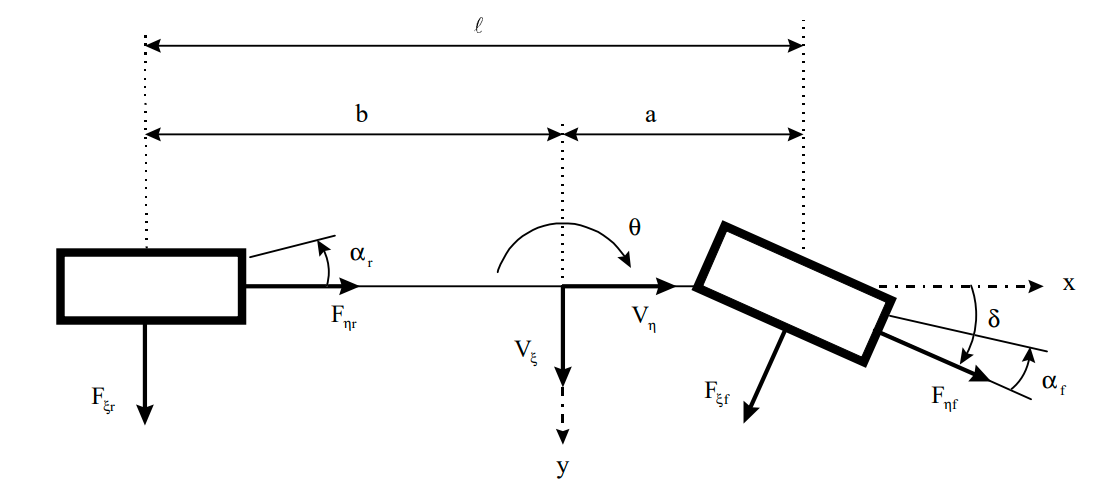
\includegraphics[width=0.5\textwidth]{figs/3dof_model_diag.png}
    \caption{3 DOF Bicycle Model}
    \label{fig:3dof_bike_model}
\end{figure}
The full nonlinear dynamics for the Bicycle model shown in \figurename{\ref{fig:3dof_bike_model}} are given as: \begin{align*}
    I \ddot{\theta}     &= a P_f \delta + b F_{\zeta f} - b F_{\zeta r}\\
    m (\dot{V_{\zeta}} + V_\eta \dot{\theta}) &= P_f \delta + F_{\zeta f} + F_{\zeta r}\\
    m(\dot{V_{\eta}} + V_\zeta \dot{\theta}) &= P_f + P_r + F_{\zeta f} \delta\\
    \dot{x} &= -V_{\zeta} \sin(\theta) + V_{\eta} \cos(\theta)\\
    \dot{y} &= V_{\eta} \cos(\theta) + V_{\zeta} \sin(\theta)
\end{align*}
where the global system coordinates are $(x, y, \theta)$, 
longitudinal $(\eta)$ and lateral $(\zeta)$ velocities $(V_\eta, V_\zeta)$,
longitudinal and lateral forces for the front and rear as $(P_f,P_r,F_{\zeta f},F_{\zeta r})$,
steering angle of $\delta$, 
and with the following physical parameters that are uncertain:

% \begin{table*}[h]
%     \centering
    \begin{tabular}{|r|l|l|}
        \hline
            & Parameter & Nominal\\
        \hline
        $m$ & Vehicle Mass & 1500.0 kg\\
        \hline
        $I$ & Vehicle Yaw Inertia & 12.0 kg m$^2$\\
        \hline
        $a$ & CG Distance to Front Axle & 1.228 m\\
        \hline
        $b$ & CG Distance to Rear Axle & 1.5618 m\\
        \hline
    \end{tabular}
% \end{table*}

There are additional complicated dynamics for how the tire forces are determined based on tire slippage and powertrain dynamics; however the simple plant model takes them as inputs.
Within the actual system actuators are used that control the steering angle and the forces that the wheels excerpt on the ground.

Within this initial simulation many assumptions are taken that will be expanded upon when analyzing the robustness to these parameters.

\textbf{Note:} 
The page limitation has made inclusion of additional details from being included. 
If desired, I can provide even more details on the system dynamics but really the 'linear' model isn't beneficial outside a single time step, although can be seen in the attached MATLAB pdf.



% \section{LPV Background}
% The following is a brief background on LPV systems:\footnote{basically a summary from the first section of \cite{ORJUELA2019295}}

% A LPV, also known as a Polytopic Model, are essentially a smooth interpolation of a set of LTI models constructed using a specified weighting function. This can be looked at as decomposing a system into multiple operating spaces that operate as linear submodels. The Polytomic Model approach takes a complex nonlinear model and spiting it as a time-varying interpolation of multiple linear submodels.\cite{ORJUELA2019295}\\

% The simple LPV structure can be described by the following weighted linear combination of LTI submodels:
% \begin{equation}\label{eq:LPV_sys_def}
% 	\begin{aligned}
% 		\dot{x}(t) 	&= \sum_{i=1}^r \mu_i(\xi(t))\{A_i x(t) + B_i u(t)\}\\
% 		y(t)		&= \sum_{i=1}^r \mu_i(\xi(t)) C_i x(t)
% 	\end{aligned}
% \end{equation}
% with state variable $x \in \real^n$ common to all submodels, control input $u \in \real^m$, output $y \in \real^p$, weighting function $\mu_i(\cdot)$ and premise variable $\xi(t) \in \real^{w}$. \cite{ORJUELA2019295} \cite{orjuela2013nonlinear}

% Additionally, the weighting functions $\mu_i (\cdot)$ for each subsystem must satisfy the convex sum constraints:
% \begin{equation}\label{eq:convex_sum_constraints}
% 	0 \leq \mu_i(\xi), \ \forall i = 1,\dots,r \ \ \text{and} \ \ \sum_{i=1} \mu_i(\xi) = 1
% \end{equation}

% %notes on dimensions: n = states, m = inputs, p = outputs, w = # of weights, r = # of subsystems

% One notable downside, for our application, is the requirement for $\xi(t)$ to be explicitly known in real-time for the model to function. This requirement is the primary driving factor in investigating this system as when $\xi(t)$ is not explicitly known additional uncertainties now exist in a system that are open for exploitation by an attacker.

% \section{Project Objectives}
% The primary objective of this project will be to reproduce three joint state and parameter estimator methods for LPV systems then test the ability of each to react to malicious input and measurement interference. A secondary/future objective will be to calculate the reachability set and how it is manipulated due to an attack on the system.

% The three estimation methods of interest\footnote{taken directly from \cite{beelen2017joint} and we are essentially recreating these results but performing additional tests} include:
% \begin{enumerate}
% 	\item Dual-Estimation (DE) approach is a method that first solves a two step optimization problem for parameters-estimation and then uses a "traditional" robust polytopic observer design for state estimation. \cite{beelen2017joint}
% 	\item Extended Kalman Filter (EKF) using prediction and update steps for the system estimates, but this version does require the assumption of Gaussian noise. \cite{beelen2017joint}
% 	\item Interacting Multiple Model estimation (IMM) method which uses a different kalmen filter for multiple modes and the probability that the system will be a certain mode.\cite{bar2004estimation}
% \end{enumerate}
% % Need to find access to \cite{bar2004estimation} for the IMM algorithm details...

% %The primary attack methods for initial testing (for simplicity) will consist of malicious random gaussian noise being added to measurements. The power of these attacks can be classified into three catagories depending on the malicous noise power:
% %\begin{enumerate}
% %	\item Stealthy attacks: power of the attack is along the same level as the normal noise standard-deviation.
% %	\item Unstealthy attacks: the attack is disruptive, yet detectable, with aims to degrade the system performance.
% %	\item Super Unstealthy attack: a very considerable attack that aims to severely disrupt a system while not remaining undetectable.
% %\end{enumerate}

% The next objective will be to show how much each attack method can effect the states (specifically the reachable set) for each estimator.\footnote{and potentially develop a better solution... modifying \cite{securestateestimation}?} This work is very similar to \cite{hashemi2018comparison} but will be expanding from stochastic DT-LTI systems to deterministic DT-LPV systems.

% \section{Proposed Methods}
% The following steps will be taken to complete the problem.

% \begin{enumerate}
% 	\item This project will begin by reproducing the results of joint state and parameter estimation from \cite{beelen2017joint} using the same LPV system used in the paper. (This will likely be done using Simulink with custom estimator blocks.)
% %	\item The next step will be to introduce additional system noise (presumably to the scheduling parameters themselves) and measurement poise into the sensors. This will be important to do first and perform a separate analysis of each before malicious attacks are included.
% 	\item Next attacks will be introduced into the sensor and the response for each estimator will be compared.
% 	\item This will then be expanded to a more interesting system\footnote{Seperator Testbed? scheduling parameters being valve on/off and for various linearized tank level systems... is it possible to analyze with a scheduling parameter dependent on a state???... Otherwise a more complicated electrical network w/ switches or pneumatic system could be done instead} that will be more useful for sensor attack testing (i.e. more sensors then states or high noise system).
% 	\item Finally, an analysis of the reachable set deviation due to attacks will be performed by finding a minimal ellipsoid constraining the states that would be reachable prior to attack detection.\footnote{possibly future work}
% \end{enumerate}

% \newpage
% \bibliographystyle{ieeetr}
% \bibliography{mybib.bib}


\end{document}
